\documentclass{article}

\usepackage[%
    left=0.5in,%
    right=0.5in,%
    top=0.5in,%
    bottom=0.5in,%
]{geometry}%
\usepackage{minitoc}
\usepackage{multicol}
\usepackage{graphicx}
\usepackage{fixltx2e}
\usepackage{listings}
\usepackage{color}
\usepackage{hyperref}
    \hypersetup{ colorlinks = true, linkcolor = blue }
\usepackage{blindtext}
\definecolor{lightgray}{gray}{0.9}
\graphicspath{ {./} }

\newcommand{\inlinecode}[2]{\colorbox{lightgray}{\lstinline
[language=#1]$#2$}}
\newcommand{\worddef}[1]{\hyperref[sec:reference]{\textit{#1}}}

\begin{document}

\tableofcontents

\newpage

\section{Designing intelligent agents}
\begin{itemize}
  \item an \worddef{agent} operates in a task environment:
  \begin{itemize}
    \item \textit{task}: the goal(s) the agent is trying to achieve
    \item \textit{environment}: that part of the real world or a computational system ‘inhabited’ by the agent 
  \end{itemize}
  \item agent obtains information about the environment in the form of percepts 
  \item agent changes the environment by performing actions to achieve its goals
\end{itemize}

\section{From agent functions to agent programs}

\begin{itemize}
  \item the \textbf{behaviour} of an agent is described by an \worddef{agent function} (action selection function) which maps a goal and sequence of percepts to an action (and possibly results)
  \item agent programming is conventionally conceived as the problem of
synthesising an agent function
  \item  Difficult to design, because of unknown environments.
\end{itemize}

\section{Agent architectures}

\begin{itemize}
  \item one way of making the agent programming problem more tractable is make use of the notion of an agent architecture 
  \item the notion of an “agent architecture” is ubiquitous in the agent literature but is not well analysed 
  \item often discussed in the context of an agent programming language or platform 
  \item architecture is a blueprint for software agents and intelligent control systems, depicting the arrangement of components
\end{itemize}

\subsection{Russell and Norvig view of an agent}

\begin{multicols}{2}

\begin{itemize}
  \item \textbf{program}: implements the agent function mapping from goals and percepts to actions (and results) 
  \item \textbf{state}: includes all the internal representations on which the agent program operates 
  \item \textbf{architecture}: computing device with sensors and actuators that runs the agent program
\end{itemize}

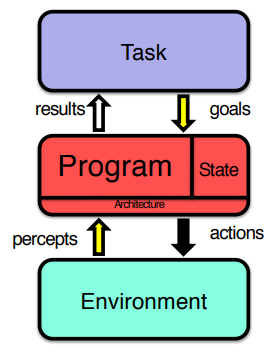
\includegraphics[scale=0.5]{russel_norvig_agent.png}

\end{multicols}

\subsection{Architecture as a virutal machine}

\begin{itemize}
  \item the architecture defines a (real or virtual) machine which runs the agent program 
  \item defines the atomic operations of the agent program and implicitly determines the components of the agent 
  \item determines which operations happen automatically, without the agent program having to do anything 
  \item e.g., the interaction between memory, learning and reasoning   
  \item an architecture constrains kinds of agent programs we can write (easily)
\end{itemize}

\pagebreak

\subsection{Architectural view of an agent} 

\begin{multicols}{2}

\begin{itemize}
  \item \textbf{program}: a function mapping from goals and percepts to actions (and results) expressed in terms of virtual machine operations 
  \item \textbf{state}: the virtual machine representations on which the agent program operates 
  \item \textbf{architecture}: a virtual machine that runs the agent program and updates the agent state
\end{itemize}

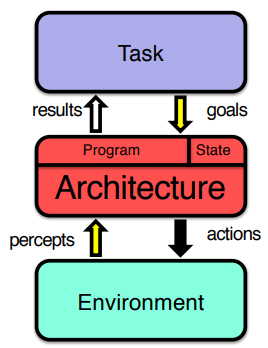
\includegraphics[scale=0.5]{architectural_agent_view.png}

\end{multicols}

\subsection{Hierarchies of virtual machines}

\begin{flushleft}
In many agents we have a whole hierarchy of virtual machines, used without qualification, ‘agent architecture’ means the most abstract architecture or the highest level virtual machine
\end{flushleft}

\section{Cognitive architecture}

\begin{itemize}
  \item agent architecture is also related to the notion of a cognitive architecture as used in artificial intelligence and cognitive science 
  \item a \textit{cognitive architecture} is an integrated system capable of supporting intelligence 
  \item often used to denote models of \textbf{human reasoning}, e.g., ACT-R, SOAR 
  \item in other cases no claims about psychological plausibility are made 
  \item in this latter sense, cognitive architecture is more or less synonymous with agent architecture as used here
\end{itemize}

\subsection{Properties of the architecture}

\begin{itemize}
  \item an agent architecture can be seen as defining a class of agent programs 
  \item just as individual agent programs have properties that make them more or less successful in a given task environment 
  \item architectures (classes of programs) have higher-level properties that determine their suitability for a task environment 
  \item choosing an appropriate architecture can make it much easier to develop an agent program for a particular task environment
\end{itemize}

\pagebreak
\section*{Reference section} \label{sec:reference}
\begin{description}
	\item[agent function] \hfill \\ The agent function is a mathematical function that maps a sequence of perceptions into action
	\item[agent] \hfill \\ In artificial intelligence, an intelligent agent (IA) is an autonomous \textbf{entity}, which observes through sensors and acts upon an environment using actuators and directs its activity towards achieving goal
\end{description}
\end{document}
